\documentclass[11pt, a4paper, oneside, portrait]{article}
\usepackage[utf8]{inputenc}
\usepackage[T2A, T1]{fontenc}
\usepackage[british, french, russian]{babel}
\usepackage[style=ieee]{biblatex}
\usepackage[most]{tcolorbox}
\usepackage{graphicx}
% \usepackage{animate}
\usepackage{xurl}
\usepackage{setspace}
\usepackage{ragged2e}
\usepackage{indentfirst}
\usepackage{mathptmx}
\usepackage{pdfpages}
\usepackage{geometry}
\usepackage{amsmath}
\usepackage{amssymb}
\usepackage{txfonts}
\usepackage{multicol}
\usepackage{fancyhdr}
\usepackage{wrapfig}
\usepackage{array}
\usepackage{float}
\usepackage{alltt}
\usepackage{tabularx}
\usepackage{caption}
\usepackage{fancyvrb}
\usepackage{fvextra}
\usepackage{enumitem}
\usepackage{bigfoot}
\usepackage{hyperref}
\geometry{
    a4paper,
    top=2cm,
    bottom=2cm,
    right=2cm,
    left=2cm
}
\hypersetup{
    colorlinks = true,
    linkcolor = blue,
    urlcolor = blue,
    filecolor = blue,
    citecolor = blue
}
\pagestyle{fancy}
\fancyhf[HC]{\textbf{MU4RBI01 --~Projet \emph{Python}}}\fancyhf[HL]{\thepage}\fancyhf[HR]{\thepage}
\fancyhf[FC]{\thepage}

\author{E{\small{}LION} G{\small{}ALIBA} Fady, N{\small{}OCHÉ} Kévin \&{} S{\small{}IVATHASAN} Ramya}
\title{\textbf{MU4RBI01 --~Projet \emph{Python}}}
\date{\today}


\begin{document}
    \selectlanguage{french}\justifying
    \maketitle

    \section*{Introduction}
        Ce présent document a pour but d'expliquer comment le projet python de l'UE \emph{MU4RBI01} de \emph{Sorbonne Université}, département scientifique, a été travaillé par le groupe n°5 de la formation d'IPS-TSDM (auteur de ce rapport).
        Pour rappel, le but de ledit projet est de créer un simple jeu de tactique, mettant en scène au moins deux joueurs, dans lequel ces derniers s'affrontent avec des unités (équivalent de soldats), tout en utilisant, dans le code source, des classes avec des liens spécifiques entre elles (relation mère-fille, etc).

        Le projet a été réalisé grâce à \emph{Github}, via l'intermédiaire de \emph{Git}.
        Les logiciels tels que \emph{Kate} ou \emph{Konsole} ont été essentiels au bon déroulement du projet. % IMPORTANT: Rajouter vos applications!

        Le repository du projet peut être retrouvé via cet URL: \url{https://github.com/NKevinVI/Sorbonne\_SdI\_IPS\_TSDM\_MU4RBI01\_Project}

    \section*{Fonctionnalités du jeu}
        \subsection*{Résumé}
            Dans le jeu, deux équipes s'affrontent: les dragons du bien (à droite de l'écran) et les dragons du mal (à gauche de l'écran).
            Les dragons du mal étant \guillemotleft{}~méchants~\guillemotright{} (Quoique?...), c'est à eux de commencer.

            Le jeu se joue un peu comme aux échecs: chaque joueur, durant son tour, fait agir une seule unité.
            Ici, chaque unité ne peut effectuer qu'une seule action par tour (à l'exception du \emph{Gueux} --~voir plus bas): se déplacer, attaquer ou effectuer sa capacité spéciale.

            Dans chaque équipe, on retrouve trois types d'unité, identiques pour chaque équipe:

            ---~Le \emph{Royal}: C'est l'unité la plus puissante.
            Elle a une vitesse de 2 (c'est-à-dire qu'elle peut se déplacer de deux cases par tour), une puissance d'attaque de 32 (elle retire 32 points de vie lors d'une attaque simple, moins la résistance de l'unité attaquée), a une résistance de 16 (chaque attaque contre elle a un malus de 16 points de dégâts, avec un minimum de zéro) et a une santé de 60 (la santé maximum).
            Elle représente le chef d'état, dirigeant (peu importe l'équipe) d'une poigne de fer ses troupes.

            ---~Le \emph{Soldat}: C'est une unité également très puissante en raison de son attaque spéciale, que nous verrons plus bas.
            Elle a une vitesse de 3, une résistance de 13, une attaque de 23 et une santé de 36.
            Dans le jeu, on lui associe l'\guillemotleft{}~aura politique~\guillemotright{} autour du \emph{Royal}, ainsi que l'immunité des élites politiques.

            ---~Le \emph{Gueux}: Cela se voit à son nom misérable, il s'agit de l'unité représentant le peuple.
            Avec une vitesse de 2, une résistance de 11, une puissance d'attaque de 17 et une santé de 23, il s'agit de l'unité la moins puissante.
            En revanche, il s'agit également de la seule unité capable de faire toutes ses actions en un tour (se déplacer, attaquer et/ou lancer sa capacité spéciale, dans n'importe quel ordre); elle est donc non négligeable.

            Chaque unité a une capacité spéciale.
            Voici ci-dessous une liste de leurs pouvoirs:

            ---~Le \emph{Royal} peut, après avoir cibler une unité, effectuer une attaque berserk contre cette unité adverse.
            L'attaque berserk inflige $1,5$ fois les dégâts ordinaires du \emph{Royal}, tout en supprimant la résistance de l'unité attaquée.
            En revanche, ce pouvoir n'est pas sans contre-partie; après avoir attaqué, le \emph{Royal} reçoit la moitié de sa puissance d'attaque en dommages plus 16, c'est-à-dire la moitié de son attaque tout en supprimant sa propore résistance aux dégâts (étant de 16).

            ---~Le \emph{Soldat} peut, lorsque sa capacité spéciale est activée, cibler une case.
            S'il attaque cette case ciblée, il inflige sa puissance d'attaque moins $4$ (soit $23-6=17$ d'attaque) à l'unité présente sur cette case. Il inflige autant de dégâts aux unités adjacentes à la case initialement touchée (sans compter les diagonales).

            ---~Le \emph{Gueux} a une technique bien à lui qui peut lui permettre de subsister plus longtemps sur le terrain: il peut se régénérer.
            Il regagne la moitié de sa puissance d'attaque en tant que points de vie, sans pouvoir cependant dépasser sa jauge maximale de santé, qui est celle fixée au tout début de la partie.

        \subsection*{Règles et Mode d'Emploi}

%     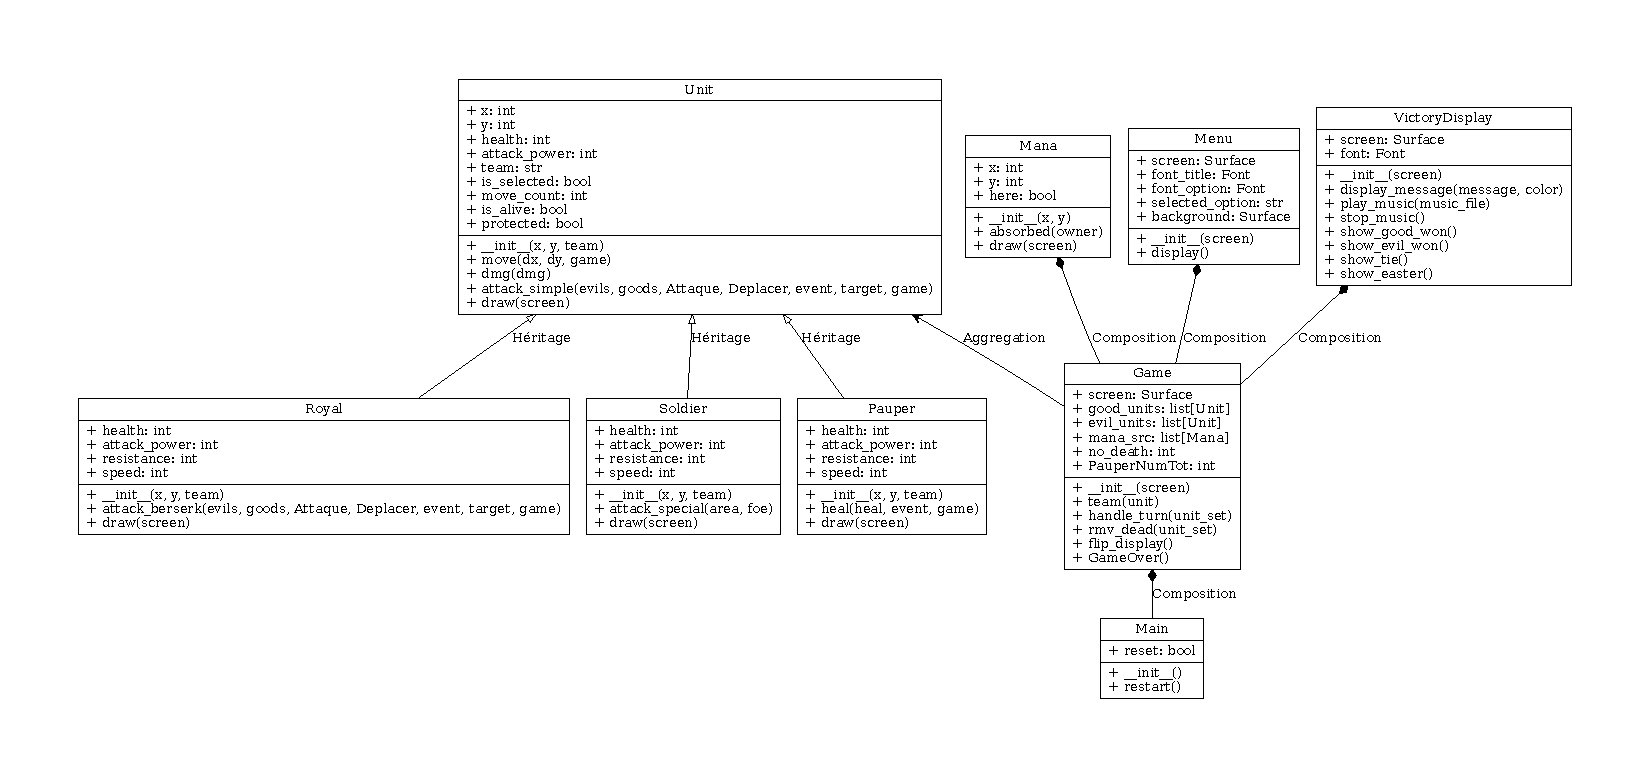
\includepdf[noautoscale=true]{UML.pdf} % À décommenter une fois le diagramme UML créé.
\end{document}
